\documentclass[11pt,a4paper]{article}

\usepackage[utf8x]{inputenc}   		% omogoča uporabo slovenskih črk kodiranih v formatu UTF-8
\usepackage[slovene]{babel}    		% naloži, med drugim, slovenske delilne vzorce

\usepackage[hyphens]{url}
\usepackage{hyperref}
\PassOptionsToPackage{hyphens}{url}	% omogoča krajšanje urljev

\usepackage{graphicx}
\usepackage{enumitem}		   		% itemsep pri enumerate

\title{Crypto finance tracker}

\author{
	Stopinšek, Amon (63150273)\\
	as7492@student.uni-lj.si\\
	\and
	Lenarčič, Istok (63150369)\\
	il4184@student.uni-lj.si\\
\ \\
Poročilo\\
Elektronsko in mobilno poslovanje \\
\\
Fakulteta za računalništvo in informatiko Univerze v Ljubljani
\date{\today}         
}



\begin{document}
\maketitle


\section{Kratek opis aplikacije}

Crypto finance tracker je Android aplikacija, ki sprejme vrednosti različnih kripto valut, ki si jih lastimo. V zameno dobimo ažurne podatke o vrednosti vsake izmed teh, ali pa vseh skupaj, v evrih. Aplikacija nudi tudi grafično predstavitev vrednosti izbrane valute v preteklosti.\\

\begin{figure}[htb]
	\begin{center}
		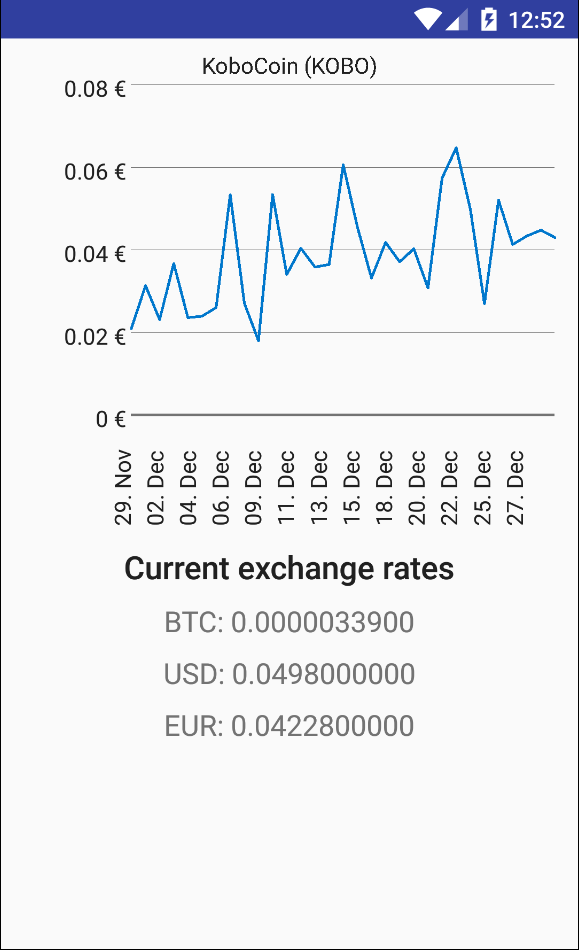
\includegraphics[width=0.8\columnwidth]{graph.png}
	\end{center}
	\caption{Crypto finance tracker}
	\label{fig:mockup}
\end{figure}

\section{Predstavitev funkcionalnosti}


\subsection{Main Activity}
Glavna aktivnost je z uporabo fragmentov razdeljena na tri dele.

\subsubsection{Fragment Wallet}
Fragment Wallet na sliki \ref{fig:wallet} je prvi fragment, ki se prikaže ob zagonu aplikacije. Prikazuje vrednost vseh vnešenih kriptovalut v evrih in bitcoinih ter
seznam vnešenih kriptovalut. 

Ob kliku na posamezno kriptovaluto se nam
odpre graf, ki prikazuje vrednost kriptovalute v zadnjih 60 dnevih.

Seznam kriptovalut se napolni s pomočjo adapterja, ki uporabi Cursor iz
poizvedbe podatkovne baze. Pred izvedbo poizvedbe se preveri ažurnost
podatkov o menjalnih tečajih. V primeru, da so podatki starejši od 5 minut
se le ti pred prikazom posodobijo s pomočjo podatkov iz APIja.

Slike kovancev kriptovalut so pridobljene preko APIja. Za prenos in 
shranjevane slik smo uporabili knjižico Picasso, ki sama poskrbi za
prenos in predpomnenje slik\cite{picasso}.


\begin{figure}[htb]
	\begin{center}
		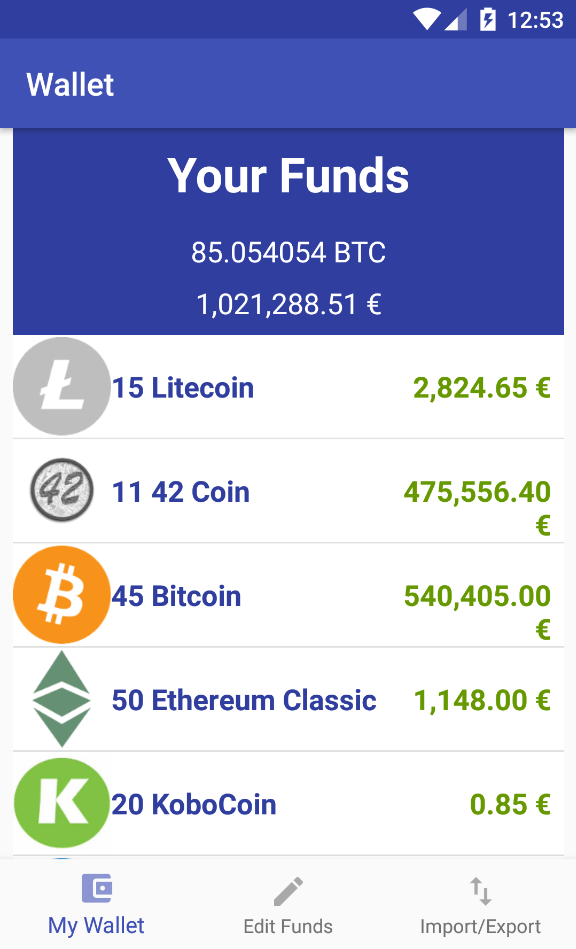
\includegraphics[width=0.8\columnwidth]{wallet.png}
	\end{center}
	\caption{Fragment Wallet}
	\label{fig:wallet}
\end{figure}

\subsubsection{Fragment Edit}
Fragment edit na sliki \ref{fig:edit_fragment} omogoča spreminjanje že vnesenih kriptovalut in dodajanje novih.

Ob pritisku na gumb za dodajanje ali izboru kriptovalute iz seznamase nam odpre 
aktivnost za urejanje, ki je prikazana na sliki \ref{fig:edit}.

Izbirno polje s seznamom kriptovalut se pridobi iz APIja. Seznam vsebuje
40 najpopularnejših kriptovalut. 

Ob shranitvi se sprememba stanja ali vnos nove kriptovalute shrani v podatkovno
bazo. Pred tem se iz APIja pridobi še menjalni tečaj. 

\begin{figure}[htb]
	\begin{center}
		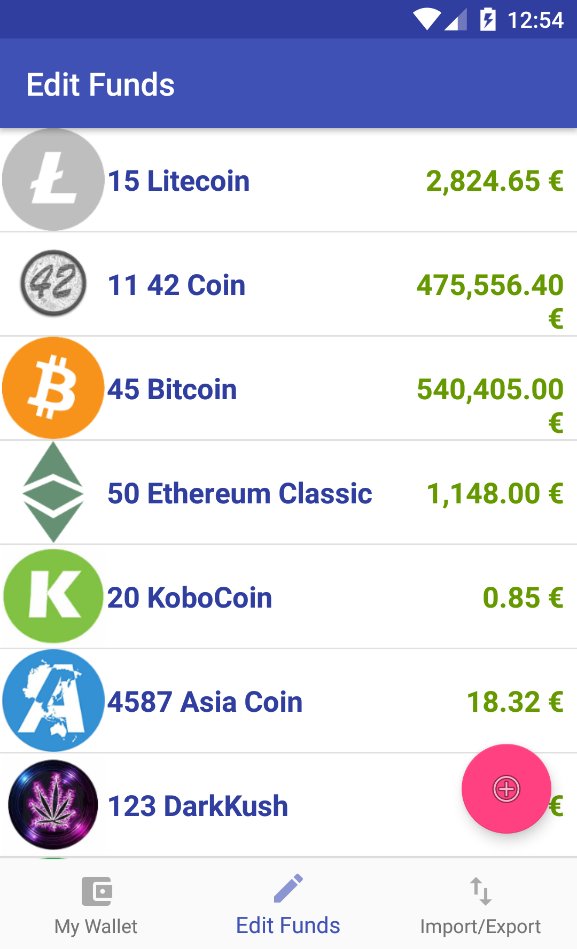
\includegraphics[width=0.8\columnwidth]{edit_funds.png}
	\end{center}
	\caption{Fragment Edit}
	\label{fig:edit_fragment}
\end{figure}

\begin{figure}[htb]
	\begin{center}
		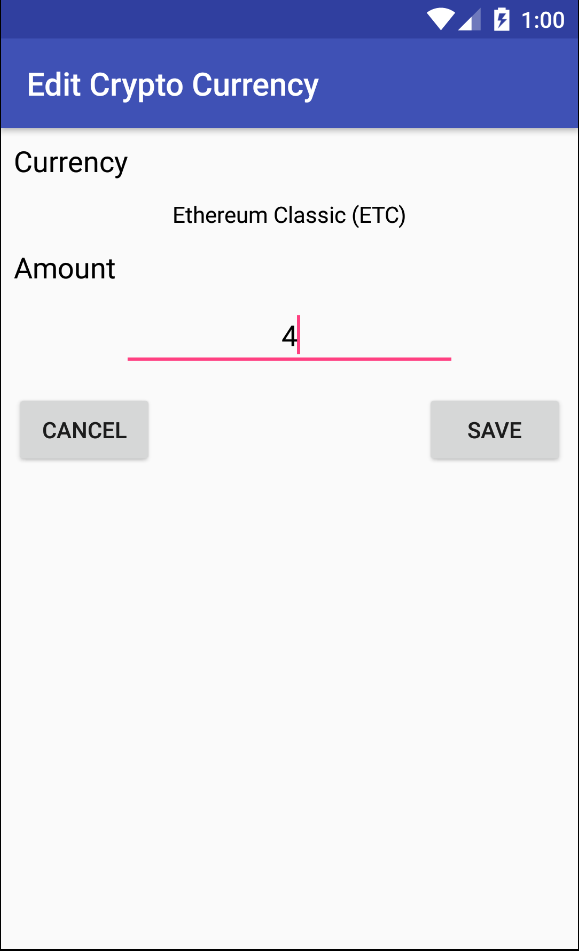
\includegraphics[width=0.8\columnwidth]{edit.png}
	\end{center}
	\caption{Activity Add/Edit}
	\label{fig:edit}
\end{figure}

\subsubsection{Fragment Import / Export}
Fragment Import / Export na sliki \ref{fig:emport_export} omogoča izvoz ali uvoz podatkovne baze.

\begin{figure}[htb]
	\begin{center}
		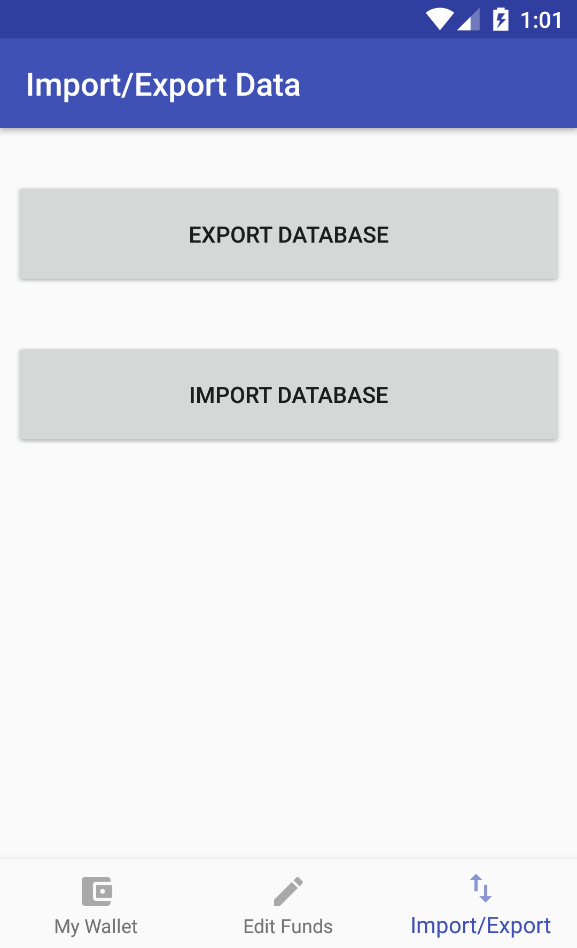
\includegraphics[width=0.8\columnwidth]{import_export.png}
	\end{center}
	\caption{Fragment Import / Export}
	\label{fig:emport_export}
\end{figure}


\subsection{Graf}

Graf na sliki \ref{fig:graph} prikazuje vrednost izbrane kriptovalute za zadnjih 60 dni. Z drsenjem
grafa levo ali desno spremenimo prikaz obdobja.

Izris grafa je narejen s pomočjo knjižice GraphView\cite{agw}.
Podatki za graf se pridobijo iz lokalne podatkovne baze. V primeru, da
so podatki v bazi starejši od 12 ur se podatki posodobijo s pomočjo 
podatkov iz APIja.

Pridobivanje podatkov in izris grafa poteka v ločeni niti. Preden se
izvajanje niti zaključi uporabniku prikažemo animacijo za nalaganje.
V primeru, da podatkov ni v bazi in jih ni mogoče pridobiti preko
APIja se uporabniku prikaže sporočilo.

Uradna dokumentacija za knjižico je skopa na področju 
oblikovanja grafa, zato smo si pri tem pomagali z vodičem\cite{gtut}.

\begin{figure}[htb]
	\begin{center}
		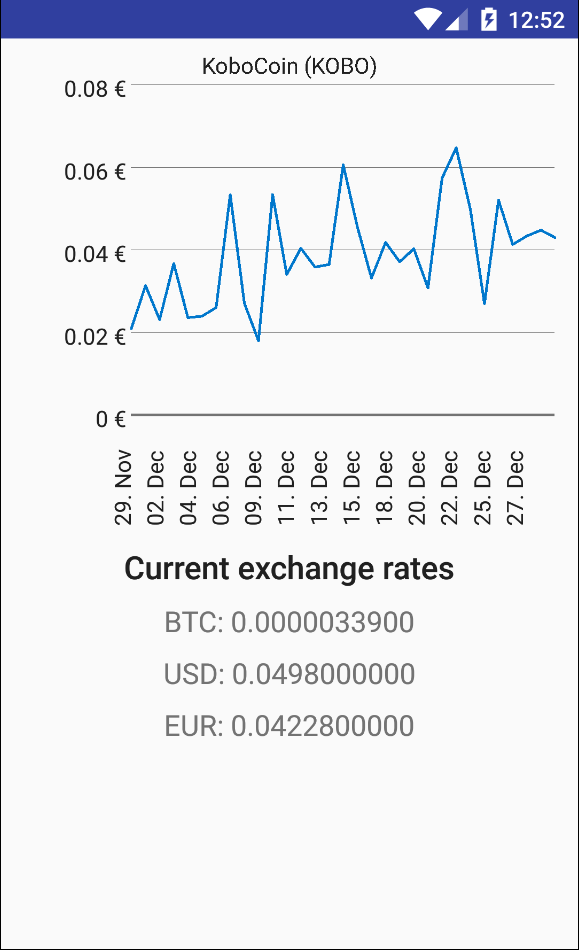
\includegraphics[width=0.8\columnwidth]{graph.png}
	\end{center}
	\caption{Graf}
	\label{fig:graph}
\end{figure}

\subsection{API}
Aplikacija vse podatke o kriptovalutah pridobi iz APIja CryptoCompare\cite{ccapi}.
Uporabljajo se naslednji zahtevki:

\begin{itemize}
\item CoinList

Vrne seznam vseh kovancev.

\item Price

Vrne trenutno ceno izbrane kriptovalute v izbranih valutah.

\item HistoDay

Vrne podatke o dnevnih vrednostih kriptovalute v izbrani valuti za izbrano obdobje.
\end{itemize}

Za delo z APIjem smo uporabili knjižico volley. Pri uporabi knjižice smo si 
pomagali s kodo iz vaj in vodiča iz uradne dokumentacije za Android\cite{volley}.

Za delo z RequestQueue smo ustvarili razred po vzorcu singelton.


\begin{thebibliography}{9}
	
	\bibitem{ccapi}
	CryptoCompare API
	\url{https://www.cryptocompare.com/api/#introduction}
	[Dostopano 15.12.2017]
	
	\bibitem{agw}
	GraphView
	\url{http://www.android-graphview.org/simple-graph/}
	[Dostopano 30.12.2017]
	
	\bibitem{gtut}
	Android Line Graph using GraphView Library Tutorial
	\url{https://www.numetriclabz.com/android-line-graph-using-graphview-library-tutorial/}
	[Dostopano 30.12.2017]
	
	\bibitem{picasso}
	Picasso - A powerful image downloading and caching library for Android
	\url{https://square.github.io/picasso/}
	[Dostopano 30.12.2017]
	
	\bibitem{volley}
	Setting Up a RequestQueue | Android Developers
	\url{https://developer.android.com/training/volley/requestqueue.html}
	[Dostopano 30.12.2017]
	
\end{thebibliography}

\end{document}  




